\section{Frequenzgang}
Polgüte $q_p$ entspricht $2\sigma = \frac{\omega_p}{q_p}$. Für identische Pole (Doppelpol, ist $\sigma_{p1} = \sigma_{p2} \xrightarrow{} q_p = \frac{1}{2}$)

\begin{align*}
	H(s) = K \cdot \frac{\prod\limits_{i=1}^{m}\overbrace{(s - z_i)}^{A_{z_1}}}{\prod\limits_{j=1}^{n}\underbrace{(s - p_j)}_{A_{p_1}}}
\end{align*}


\noindent\textbf{Beispiel}
\[
H(s) = \frac{1}{s^2 + \underbrace{\frac{s}{4}}_{\frac{\omega_p}{q_p} = 2 \zeta \omega_p^2} + \underbrace{1^2}_{\omega_p^2}}
\]

\begin{center}
	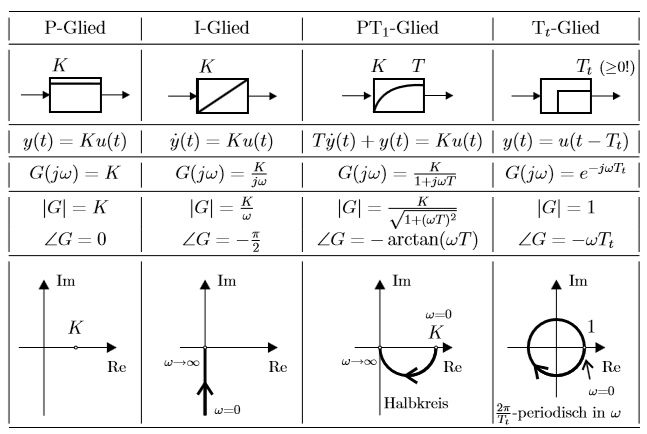
\includegraphics[width=\columnwidth]{Images/frequenzgang_grundglieder}
\end{center}


\subsection{Zeigerdiagramm}
\script{116}

\subsection{Bodediagram}
\noindent\textbf{Beispiel}
Diagram zu $G(j\omega) = \frac{2}{j\omega}\cdot \frac{1}{(0.5j\omega + 1)^2}$
\begin{center}
	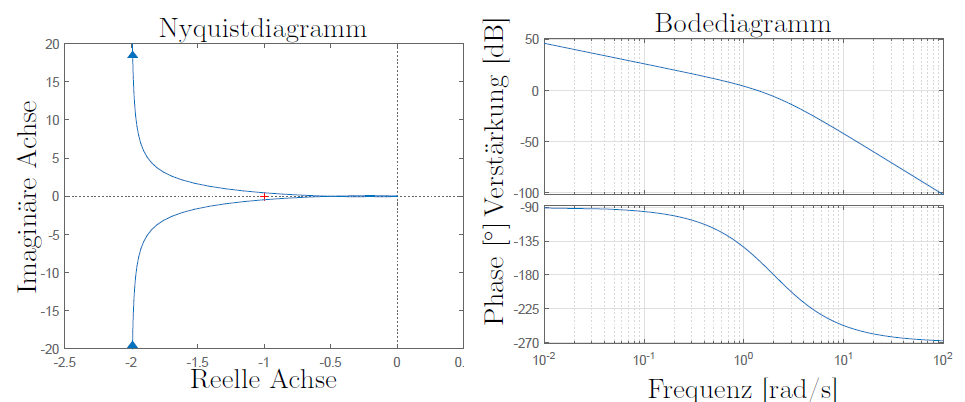
\includegraphics[width=\columnwidth]{Images/bode}
\end{center}


\subsubsection{Bel}\script{131}
[B] (Bel) ist ein $\log_{10}$ einer Leistung. Meist wird in Regeleungstechnik folgende Berechnung verwendet:
\[k_{\text{P}} = 20 \cdot \log_{10}\left(\frac{G_y}{G_x}\right) \qquad [dB]\]


\subsection{Nyquist Diagramm}
Nyquist zeichnen durch bestimmen einiger Eckpunkte:
\begin{enumerate}[nosep]
	\item $\lim\limits_{\omega \rightarrow 0}H(j\omega)$
	\item $\lim\limits_{\omega \rightarrow \infty}H(j\omega)$
	\item $\Re[H(j\omega)] = 0$
	\item $\Im[H(j\omega)] = 0$
\end{enumerate}
Ende zB $j\omega$ kommt von unten, pro $j\omega$ Potenz ergibt dies eine Drehung um $90^\circ$. (e.B $s^2$ von links)
~\\
\textbf{Hinweis}: Pole in der Nähe der linken Im-Achse sind schnelle Bewegungen, gegen $-\infty$ langsam. Wenn Doppel-Pol genau auf der Im-Achse liegt, ist die Dämpfung 0, aber die Eigenfrequenz wird unendlich gross.


\subsection{Nyquistkriterium - Stabilität}
\begin{center}
\textit{Die Idee ist, Informationen über den offenen Regelkreis zu benutzen, um die Stabilität des geschlossenen Regelkreises zu beurteilen. \script{126}}
\end{center}
Mithilfe des Nyquist-Diagramm (Ortskurve) kann die Stabilität eines Systems überprüft werden.
\begin{itemize}[nosep]
	\item Gemäss folgender Abbildung wird $G_0 = \prod_{i}G_i$ gebildet aus den seriegeschalteten Teilsystemen des offenen Regelkreises (Rückwärtspfad unterbrechen bei $Y_4$).
	\item $G_0$ muss dabei einem Prozess mit Ausgleich entsprechen; d.H. maximal zwei Pole bei Null und alle weiteren Pole müssen in der linken Halbebene liegen.
	\item Damit der geschlossene Regelkreis stabil ist, muss der \textbf{kritische Punkt $-1$ links der Nyquistkurve} von $G_0$ liegen. wenn diese in Richtung zunehmender Frequenz durchlaufen wird. $(\omega = 0\dots\omega)$
\end{itemize}

\begin{center}
	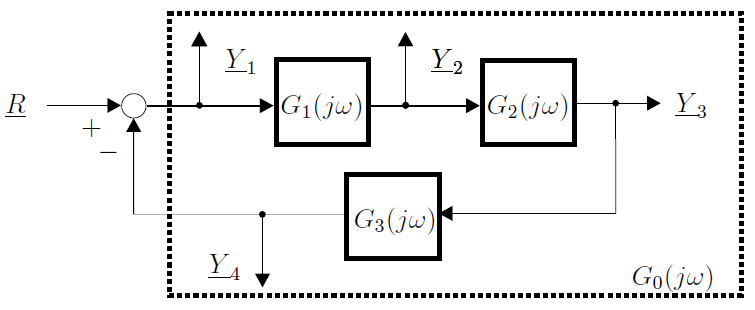
\includegraphics[width=\columnwidth]{Images/kreisschaltung}\\
\end{center}

\subsubsection{Reserven}
\script{128} Phasenreserve $\Phi = 40\dots70$, Verstärkungsreserve $K > 4 (\approx 12dB)$, Totzeit bringt normalerweise nur Nachteile
\begin{center}
	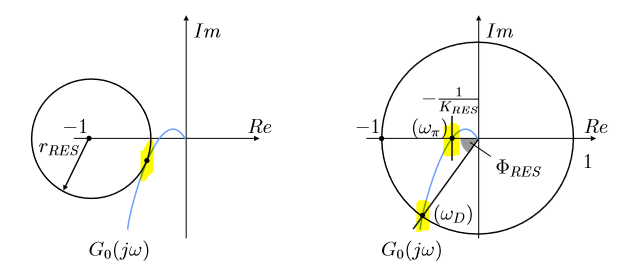
\includegraphics[width=\columnwidth]{Images/reserve}
\end{center}
\textbf{Durchtrittsfrequenz} $\omega_D$ entspricht $\left|G_0(j\omega_D)\right| = 1$.\\
\textbf{Phasenschnittfrequenz} $\omega_\pi$ entspricht $\Im(G_0(j\omega_\pi)) = 0$~\\

\noindent Der Regelkreis ist stabil, wenn einer der Bedingungen zutrifft \script{127}:
\begin{itemize}[nosep]
	\item $\omega_\pi > \omega_D$
	\item $G_0(j\omega_D) = e^{-j\varphi}$ mit $0 < \varphi < \pi$
	\item $0 > G_0(j\omega_\pi) > -1$
\end{itemize}
~\\

\noindent\textbf{Einstellen nach Phasenreserve}
\begin{enumerate}[nosep]
	\item $\arg(G_0(j\omega_D)) = -\pi + \Phi_{res}$, Durchtrittsfrequenz $\omega_D$ bestimmen
	\item $\left|G_0(j\omega_D)\right| = 1$, auflösen nach $K_R$
\end{enumerate}
~\\
\noindent\textbf{Einstellen nach Verstärkungsreserve} $K_{Rres}$
\begin{enumerate}[nosep]
	\item $\omega_\pi$ aus $\arg(G_0(j\omega_\pi)) = -\pi$ oder $\Im(G_0(j\omega_\pi)) = 0$ berechnen
	\item $K_R = \frac{1}{K_{Rres} \cdot \left|G_0(j\omega_\pi)\right|}$,  wobei bei $\left|G(j\omega_\pi)\right| \rightarrow K_R = 1$ gewählt
\end{enumerate}~\\


\subsubsection{DGL Stabilität}\script{140}
Wenn die stabilität von einem LZI DGL mit Eingang $u$ und Ausgang $y$ untersucht werden soll, kann das charakteritische Polynom verwendet werden. Dabei müssen alle $\lambda$ auf der Linken-Halbenene liegen. \textbf{Tip:} Für einfache System von 1. und 2. Ordnung müssen alle Koeffizienten des chara. Polynom das selbe Vorzeichen haben, um stabil zu sein. $u$ ist dabei irrelevant.

\subsubsection{Bode Stabilität}
\script{138} Im Bode Diagram sind $\omega_\pi$ (Schnitt mit $-180^\circ$) und $\omega_D$ (Schnitt mit $0dB$) einfach zu bestimmen. Durch ablesen im Bode Diagram können Phasenreserve $\Phi_{res} = 21.4^\circ$ und Verstärkungsreserve $K_{res} = 6dB = 2$ abgelesen werden.
\begin{center}
	\includegraphics[width=\columnwidth]{Images/bode_stabilität}
\end{center}

\subsection{Mason's Regel}
UTF von $x_i$ nach $x_j$ , wobei $x_i$ eine Quelle, $x_j$ jedoch nicht zwingend eine Senke sein muss.
\[
H_{ij} = \frac{\sum_{k}P_k\cdot\Delta_k}{\Delta}
\]
$P_k \Rightarrow$ Vorwärtspfad $k$ (bezogen auf 1 Eingang)\\
$\Delta_k \Rightarrow $ 1 - (Summe alle Schleifen die $P_k$ nicht berühren) + (Summe aller Produkte zweier Schleifen, die $P_k$ und sich selbst nicht berührenn) - (Summe aller Produkte dreier Schleifen, die $P_k$ und sich selbst nicht berührenn) + $\dots$\\
$\Delta \Rightarrow $ 1 - (Summe alle Schleifen) + (Summe aller Produkte zweier Schleifen, die sich nicht berühren) - (Summe aller Produkte dreier Schleifen, die sich nicht berühren) + $\dots$\\
~\\ \textbf{Beispiel}\\
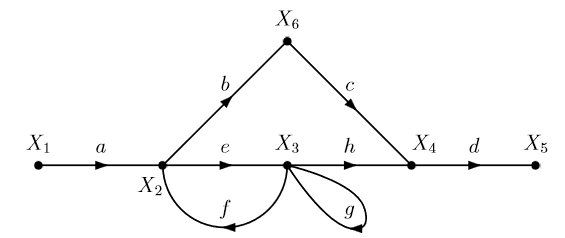
\includegraphics[width=\columnwidth]{Images/sfd_beispiel}
Die UTF zwischen $x_1$ und $x_4$ ist mit Mason's Regel:
\[
H_{1,4} = \frac{x_4}{x_1} = \frac{aeh \cdot 1 + abc - abcg}{1 - ef - g}
\]

